\part{DNN Verification Algorithms}
\chapter{Search Algorithms}

\section{Branch-and-Bound (BaB)}\label{sec:bab}

    
\SetKwData{nextlayer}{layer$_{i+1}$}
\SetKwData{status}{status}
\SetKwData{minimum}{objval}

\SetKwFunction{InputMILP}{AddInputConstrs}
\SetKwFunction{GetUnstableNeurons}{GetUnstableNeurons}
\SetKwFunction{PiecewiseLinearMILP}{AddConstrsPWL}
\SetKwFunction{LinearMILP}{AddConstrsLinear}
\SetKwFunction{Maximize}{Maximize}
\SetKwFunction{Minimize}{Minimize}
\SetKwFunction{Feasible}{CheckFeasibility}
\SetKwFunction{Optimize}{Optimize}
\SetKwFunction{isPiecewiseLinear}{isPiecewiseLinear}
\SetKwFunction{CreateStabilizedMILP}{CreateStabilizedMILP}
\SetKwFunction{GetLeafNodes}{GetLeafNodes}
\SetKwFunction{AddConstrs}{AddConstrs}
\SetKwFunction{RemoveConstrs}{RemoveConstrs}
\SetKwFunction{AddObjective}{AddObjectives}
\SetKwFunction{ShortenSplitConstrs}{ShortenSplitConstrs}
\SetKwFunction{RemoveLeafNodes}{RemoveLeaves}
\SetKwFunction{StoppingConditions}{StoppingConditions}
\SetKwFunction{RepOK}{RepOK}
\SetKwFunction{RaiseError}{RaiseError}

\SetKwInOut{Input}{input}
\SetKwInOut{Output}{output}
\SetKw{Break}{break}
\SetKw{Continue}{continue}
\SetKwFunction{Backtrack}{Backtrack}
\SetKwFunction{Select}{Select}
\SetKwFunction{Decide}{Decide}
\SetKwFunction{BCP}{BCP}
\SetKwFunction{Deduce}{Deduce}
\SetKwFunction{AnalyzeConflict}{AnalyzeConflict}
\SetKwFunction{BooleanAbstraction}{BooleanAbstraction}
\SetKwFunction{AddClause}{AddClause}
\SetKwFunction{isTotal}{isTotal}
\SetKwFunction{randomattack}{RandomAttack}
\SetKwFunction{pgd}{PGDAttack}

\SetKwFunction{DPLLT}{DPLLT}
\SetKwFunction{isValid}{isValid}
\SetKwFunction{isEmpty}{isEmpty}
\SetKwFunction{LPSolver}{LPSolver}
\SetKwFunction{Solve}{Solve}
\SetKwFunction{FindLayerNodes}{FindLayerNodes}
\SetKwFunction{TightenInputBounds}{TightenInputBounds}
\SetKwFunction{Abstract}{Abstract}
\SetKwFunction{Check}{Check}
\SetKwFunction{Decide}{Decide}
\SetKwFunction{Imply}{Imply}
\SetKwFunction{Lower}{LowerBound}
\SetKwFunction{Upper}{UpperBound}
\SetKwFunction{GetInputBounds}{GetInputBounds}
\SetKwFunction{GetInputs}{GetInputs}
\SetKwFunction{GetNumInputs}{GetNumInputs}
\SetKwFunction{CurrentConflictClause}{CurrentConflictClause}
\SetKwFunction{StopCriterion}{StopCriterion}
\SetKwFunction{LastAssignedLiteral}{LastLiteral}
\SetKwFunction{LiteralToVariable}{LiteralToVariable}
\SetKwFunction{Antecedent}{Antecedent}
\SetKwFunction{BinRes}{BinRes}
\SetKwFunction{BacktrackLevel}{BacktrackLevel}
\SetKwFunction{AddClause}{AddClause}
\SetKwFunction{ActivationStatus}{ActivationStatus}
\SetKwFunction{Backjump}{Backjump}
\SetKwFunction{EstimateBounds}{EstimateBounds}

\SetKwData{problems}{ActPatterns}
\SetKwData{implicationgraph}{igraph}
\SetKwData{literal}{lit}
\SetKwData{variable}{var}
\SetKwData{antecedent}{ante}
\SetKwData{conflict}{conflict}
\SetKwData{none}{none}
\SetKwData{layerid}{lid}
\SetKwData{hiddenbounds}{hidden\_bounds}
\SetKwData{inputs}{inputs}
\SetKwData{inputbounds}{input\_bounds}
\SetKwData{outputbounds}{output\_bounds}
\SetKwData{infeasible}{INFEASIBLE}
\SetKwData{unreachable}{UNREACHABLE}
\SetKwData{maxinputs}{MAX\_NUM\_INPUT}
\SetKwData{assignment}{$\sigma$}
\SetKwData{dl}{dl}
\SetKwData{lpmodel}{solver}
\SetKwData{clauses}{clauses}
\SetKwData{conflict}{conflict}
\SetKwData{clause}{clause}
\SetKwData{igraph}{igraph}
\SetKwData{cex}{cex}
\SetKwData{sat}{sat}
\SetKwData{unsat}{unsat}

\SetKwData{submodel}{sub\_model}

\SetKwData{true}{true}
\SetKwData{false}{false}
    
\SetKwFunction{Restart}{Restart}

\SetKwData{counterexample}{cex}
\SetKwData{conflictclause}{conflict\_clause}
\SetKwData{isconflict}{is\_conflict}


\begin{algorithm}[t]
    \footnotesize
    \Input{DNN $\mathcal{N}$, property $\phi_{in} \Rightarrow \phi_{out}$}
    \Output{$\unsat$ if property is valid, otherwise ($\sat, \counterexample$)}
    \BlankLine

    $\problems \leftarrow \{ \emptyset \}$ \tcp{initialize verification problems} 
    % $\prooftree \gets \{ ~ \}$ \tcp{initialize proof tree}\label{line:prooftree}
    
    \While(\tcp*[h]{main loop}){$\problems$}{\label{line:dpllstart}
        % \tcp{$\sigma_i$ is the activation pattern of problem $i$-th}
        $\sigma_i \gets \Select(\problems)$ \tcp{process problem $i$-th}
        % \Parfor(\tcp*[h]{process in parallel}){$\sigma_i ~\In~ \problems$}{ \label{line:parfor}
            \If{\Deduce{$\mathcal{N}, \phi_{in}, \phi_{out}, \sigma_i$}}{\label{line:deduce}
                $(\counterexample, v_i) \leftarrow \Decide(\mathcal{N}, \phi_{in}, \phi_{out}, \sigma_i)$ \\ \label{line:decide}
                \If(\tcp*[h]{found a valid counter-example}){$\counterexample$}{
                    \Return{$(\sat, \counterexample)$} 
                }
                \tcp{create new activation patterns}
                $\problems \leftarrow \problems \cup \{ \sigma_i \land v_i ~;~ \sigma_i \land \overline{v_i} \}$ \;
            }
            %\Else(\tcp*[h]{detect a conflict}){
                % $\clauses \leftarrow \clauses \cup \AnalyzeConflict(\igraph_i)$ \\ \label{line:analyze_conflict}
            %    $\prooftree \leftarrow \prooftree \cup \{ \sigma_i \}$ \tcp{build proof tree} \label{line:record_proof}
            %}
        % }
        % \If(\tcp*[h]{no more problems}){$\isEmpty(\problems)$}{
        % }
        
    }\label{line:dpllend}
    \Return{\unsat}
    
    \caption{The \bab{} algorithm.}\label{alg:bab}
\end{algorithm}

Most modern DNN verifiers adopt the branch-and-bound (BaB) approach to search for activation patterns for DNN verification. A BaB search consists of two main components: (branch) splitting into the problem smaller subproblems 
by using \emph{neuron splitting}, which decides boolean values representing neuron activation status, 
and (bound) using abstraction and LP solving to approximate bounds on neuron values to determine 
the satisfiability of the partial activation pattern formed by the split.


\autoref{alg:bab} shows \bab{}, a reference BaB architecture~\cite{nakagawa2014consolidating} for modern DNN verifiers. \bab{} takes as input a ReLU-based DNN $\mathcal{N}$ and a formulae $\phi_{in}\Rightarrow \phi_{out}$ representing the property of interest.
\bab{} iterates between (i) branching (\autoref{line:decide}), which \emph{decides} (assigns) an activation status value for a neuron, and (ii) bounding (\autoref{line:deduce}), which \emph{deduces} or checks the feasibility of the current activation pattern. 
%To add proof generation capability, \bab{} is instrumented with a proof tree (\texttt{proof}) variable (\autoref{line:prooftree}) to record these branching decisions. The proof is represented as a binary tree structure, where each node represents a neuron and its left and right edges represent its activation decision (active or inactive). %The proof tree is then used to generate a proof in the \prooflang{} format (\autoref{sec:proof-format}).




\begin{figure}[t]
    \centering
    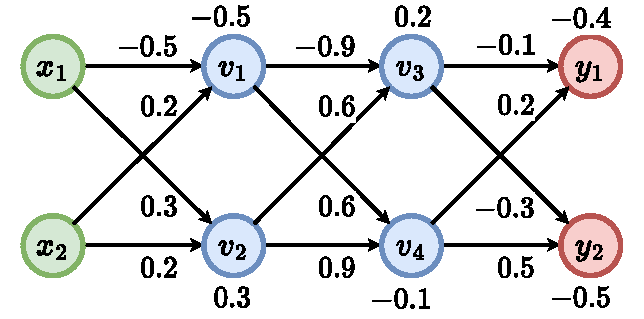
\includegraphics[width=0.5\linewidth]{figure/proof_net.pdf}
    \caption{(a) A simple DNN (a redrawn of~\autoref{fig:example1})  (b) A proof tree produced verifying the property $(x_1, x_2) \in [-2.0, 2.0] \times [-1.0, 1,0] \Rightarrow (y_1 > y_2)$.}\label{fig:example1}
\end{figure}
%White nodes correspond to branching nodes where \neuralsat{} makes decisions to split ReLU neurons.

\paragraph{Example} \autoref{fig:example1}a illustrates a DNN and how \bab{} verifies that this DNN has the property $(x_1, x_2) \in [-2.0, 2.0] \times [-1.0, 1,0] \Rightarrow (y_1 > y_2)$. 

First, \bab{} initializes the activation pattern set \functiontextformat{ActPatterns} with an empty activation pattern $\emptyset$. Then \bab{} enters a loop (\autoref{line:dpllstart}-\autoref{line:dpllend}) to search for a satisfying assignment. In the first iteration, \bab{} selects the only available activation pattern $\emptyset \in \functiontextformat{ActPatterns}$. 
It calls \functiontextformat{Deduce} to check the feasibility of the problem based on the current activation pattern. \functiontextformat{Deduce} uses abstraction to approximate that from the input constraints the output values are feasible for the given network. 
Since \functiontextformat{Deduce} cannot decide infeasibility, \bab{} randomly selects a neuron to split (\functiontextformat{Decide}). Let us assume that it chooses $v_4$ to split, which essentially means the problem is split into two independent subproblems: one with $v_4$ active and the other with $v_4$ inactive.
\bab{} then adds $\{v_4\}$ and $\{\overline{v_4}\}$ to \functiontextformat{ActPatterns}.

In the second iteration, \bab{} has two subproblems (that can be processed in parallel). For the first subproblem with $v_4$, \functiontextformat{Deduce} cannot decide infeasibility, so it selects $v_2$ to split. It then conjoins $v_4$ with $v_2$ and then with $\overline{v_2}$ and adds both conjuncts to \texttt{ActPatterns}. 
For the second subproblem with $\overline{v_4}$ inactive, \functiontextformat{Deduce} determines that the problem is unsatisfiable.

In the third iteration, \bab{} has two subproblems for $v_4 \land v_2$ and $v_4 \land \overline{v_2}$. For the first subproblem, \functiontextformat{Deduce} cannot decide infeasibility, so it selects $v_1$ to split. It then conjoins $v_1$ and then $\overline{v_1}$ to the current activation pattern and adds them to \functiontextformat{ActPatterns}. For the second subproblem, \functiontextformat{Deduce} determines that the problem is unsatisfiable.

In the fourth iteration, \bab{} has two subproblems for $v_4 \land v_2 \land v_1$ and $v_4 \land v_2 \land \overline{v_1}$. Both subproblems are determined to be unsatisfiable.

Finally, \bab{} has an empty \texttt{ActPatterns}, stops the search, and returns \texttt{unsat}.




